\begin{figure}[H]
    \centering
    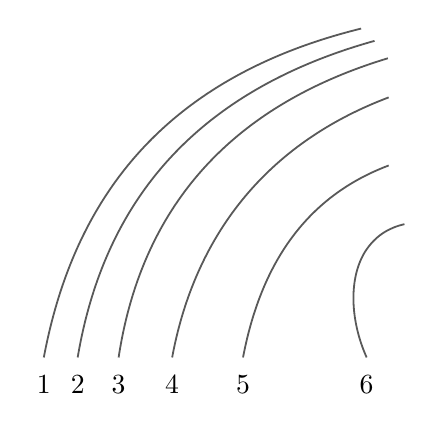
\begin{tikzpicture}[x=1.0cm,y=0.92cm]
        \tikzset{level curve/.style={draw=black!65, line width=0.65pt}}

        \draw[level curve]
            (-2.65,0.12)
            .. controls (-2.30,2.14) and (-1.27,3.95) .. (1.38,4.66);
        \draw[level curve]
            (-2.22,0.12)
            .. controls (-1.92,2.05) and (-0.92,3.74) .. (1.55,4.49);
        \draw[level curve]
            (-1.70,0.12)
            .. controls (-1.45,1.91) and (-0.53,3.51) .. (1.72,4.25);
        \draw[level curve]
            (-1.02,0.12)
            .. controls (-0.76,1.65) and (0.05,3.02) .. (1.73,3.71);
        \draw[level curve]
            (-0.12,0.12)
            .. controls (0.08,1.26) and (0.58,2.30) .. (1.73,2.77);
        \draw[level curve]
            (1.45,0.12)
            .. controls (1.24,0.63) and (1.22,1.21) .. (1.43,1.58)
            .. controls (1.56,1.80) and (1.73,1.91) .. (1.93,1.96);

        \node[below] at (-2.65,0) {$1$};
        \node[below] at (-2.22,0) {$2$};
        \node[below] at (-1.70,0) {$3$};
        \node[below] at (-1.02,0) {$4$};
        \node[below] at (-0.12,0) {$5$};
        \node[below] at (1.45,0) {$6$};
    \end{tikzpicture}
    \caption{The second family of level curves in Exercise 3.2.}
    \label{fig:exercise-3-2-level-sets-b}
\end{figure}
